\chapter{\SysName アルゴリズム}
本章において,\$1を拡張した\$Vアルゴリズムを述べる.

\section{\$Vアルゴリズムが目指す特徴}
\$Vアルゴリズムが目指す特徴を以下に示す.
\begin{itemize}
\item \$1の特徴を維持すること.つまり,
\begin{itemize}
\item ハードウェアやソフトウェアのセンシング及び入力する速度などによって変わるサンプリングされる点の数の違いに対してロバストであること.
%\item 手書きジェスチャの大きさ,向き,位置の不変に関してオプショナルに設定可能であること.
\item 数学的な高度な知識やテクニックをを必要としないこと~(例えば,逆行列,微分,積分など)
\item 少ないコードによって実装できること.
\item 認識速度が速いこと.
\item ソフトウェア開発者やアプリケーションユーザが,独自に手書きジェスチャを定義できること.
\item N-best listに関して,高い識別能力を示すスコアを示すこと.
\item 図\ref{fig:stroke_1}のような単一ストロークからなる手書きジェスチャを認識するにあたり,HCI分野において多く用いられる既存の複雑な手書きジェスチャ認識アルゴリズムと比べても,高い認識率を示すこと.
\end{itemize}
\item 前項目を満たした上で,形状や書き順が同じ手書きジェスチャを大きさ,向き,位置に関して識別可能にすること.
\end{itemize}

これまで述べてきたように,一般的に,特徴量を不変にすることによってその特徴量についてロバスト性が向上する.しかしながら,不変にしない場合,つまり,認識に用いる特徴量として扱う場合,ロバスト性が低下し,結果的に認識率の低下を招く恐れがある.つまり,\$1アルゴリズムを踏襲した上で,大きさ,向き,位置を特徴量として用い,それらに関して識別可能にするということは,\$1と比べて,認識率が低下すると言える.
以上を踏まえ,\$1に比べて,認識率や認識速度を著しく損なうことなく,図\ref{fig:examples_V}のような,手書きジェスチャの形状と書き順は同じでも,大きさ,向き,位置が異なるジェスチャを識別するアルゴリズムを実現することが\$Vの目指すところである.

\section{\$Vアルゴリズムのアイディア}
ここでは,\$Vアルゴリズムのアイディアを述べる.

まず,形状や書き順が同じ手書きジェスチャを大きさ,向き,位置に関して識別可能にする方法について述べる.次に,\$1において認識できなかった1次元の手書きジェスチャを認識する方法について述べる.そして,\$Vアルゴリズムの最大の特徴である,学習データの保持の方法について述べる.

\subsection{大きさ,向き,位置に関して識別可能にする方法}
\$1アルゴリズムを活用し,ジェスチャを大きさ,向き,位置によって識別可能にするための方法として以下の2つが考えられる.
\begin{enumerate}
\item 単純にリサンプリングした点のみによって判別する~(正規化しない).
\item 正規化した上で,それぞれを特徴量として用いる.
\end{enumerate}
1. の場合,リサンプリングしただけの実質生データのまま比較するため,大きさ,向き,位置によって識別可能となる.しかしながら,手書きジェスチャの場合,アプリケーションユーザの入力は毎度微妙に異なることが予想される.そのため,類似したジェスチャにおいても,類似度が低くなり,ロバスト性が低下する恐れがあるとともに,認識されたか否かを判別するための類似度の閾値の設定が困難になることが予想される.
2. の場合,ジェスチャを正規化するためロバスト性は維持され,その上で,大きさ,向き,位置を特徴量として用いるため,1. の場合と比べて,類似度が低くなりづらくなると予想される.
そこで,\$Vは2. の方法を用いることとする.

\subsection{1次元の手書きジェスチャを認識する方法}
\$Vは\$1とは異なり,1次元の手書きジェスチャを認識できるようにした.これは\$N\cite{}において実装されているため,\$Nにおいて用いられている方法を用いる.
具体的には,\$1において大きさを正規化する際に用いられる,手書きジェスチャに隣接する矩形の縦の長さが横の長さに対し~(あるいはその逆が) 0.3未満の長さであれば,その手書きジェスチャは大きさに正規化しない.これにより,1次元の手書きジェスチャを認識することが可能となる.

\subsection{学習データの保持の方法}
\$Vは学習データの保持の方法において特徴がある.

\$Vは学習データが追加されるたびに,ジェスチャの形状と書き順が同じ学習データを同じグループに分類する.ここでは形状と書き順が同じジェスチャを識別可能な\$1アルゴリズムを用いている.この形状と書き順に従って分類されたジェスチャを``ジェスチャグループ''と名付ける.ジェスチャグループの例を図に示す~(あるいは図\ref{fig:examples_V}もジェスチャグループの例である).

このようにジェスチャグループを作成する理由は2つある.
\begin{itemize}
\item 認識速度の低下を防ぐため.
\item 認識率の低下を防ぐため.
\end{itemize}
それぞれについて理由を述べる.


\subsubsection{ジェスチャグループの作成が認識速度の低下を防ぐ理由}

大きさ,向き,位置を特徴量として認識に用いる場合,それぞれについての類似度計算を行うこととなる.これを全てのジェスチャについて類似度計算を行った場合,認識速度が低下する要因となる.
\$Vの目的は,ジェスチャの形状と書き順が同じであるが,大きさ,向き,位置に関して識別可能にすることである.そこで,形状と書き順が同じジェスチャが集まったジェスチャグループを作成し,ジェスチャグループ内に存在する学習データのみに対し,大きさ,向き,位置の類似度計算をする~(\TODO{ここら辺がわかりやすくなるような,入力データと複数のジェスチャグループからなる図を作成する}).一般的に,認識速度は,認識に用いる特徴量を増やした場合,増やさない場合と比べて,学習データの数に比例してその差が大きくなるが,同一ジェスチャグループ内のみに対し認識に用いる特徴量を増やすことによって,全体的な認識速度の低下を防ぐことが可能となると考え,我々は「ジェスチャグループを作成し,ジェスチャグループ内に存在する学習データのみに対し,大きさ,向き,位置の類似度計算をすると認識速度の低下を抑えることができる」という仮説を立てた.

\subsubsection{ジェスチャグループの作成が認識率の低下を防ぐ理由}

大きさ,向き,位置の特徴量を認識のために全てのジェスチャに対し用いた場合を考える.
例えば,図\ref{fig:cannot_recognized}Aの場合について考える.
学習データ~(図\ref{fig:cannot_recognized}A')が図\ref{fig:cannot_recognized}Aの右下のジェスチャと一致させようと入力されたとする.しかし,この2つのジェスチャは大きさが異なるため,大きさを認識のための特徴量として用いている限り類似度が低下し認識率が下がることが考えられる.また,これはロバスト性の低下につながる.

図\ref{fig:cannot_recognized}Bの場合について考える.
学習データ~(図\ref{fig:cannot_recognized}B')が図\ref{fig:cannot_recognized}Bの右のジェスチャと一致させようと入力されたとする.しかし,この2つのジェスチャは向きが異なるため,向きを認識のための特徴量として用いている限り類似度は低下し認識率が下がることが考えられる.また,これはロバスト性の低下につながる.

図\ref{fig:cannot_recognized}Cの場合について考える.
学習データ~(図\ref{fig:cannot_recognized}C')が図\ref{fig:cannot_recognized}Cのジェスチャと一致させようと入力されたとする.しかし,この2つのジェスチャは大きさ,向き,位置が異なるため,大きさ,向き,位置を認識のための特徴量として用いている限り類似度は低下し認識率が下がることが考えられる.また,これはロバスト性の低下につながる.

これまでに述べてきたが,大きさ,向き,位置を認識のための特徴量として新たに用いることによって,それぞれについてロバスト性が低下,つまり,認識率の低下を招く恐れがある.図\ref{fig:cannot_recognized}はその例である.

\begin{figure} [h!]
	\begin{center}
		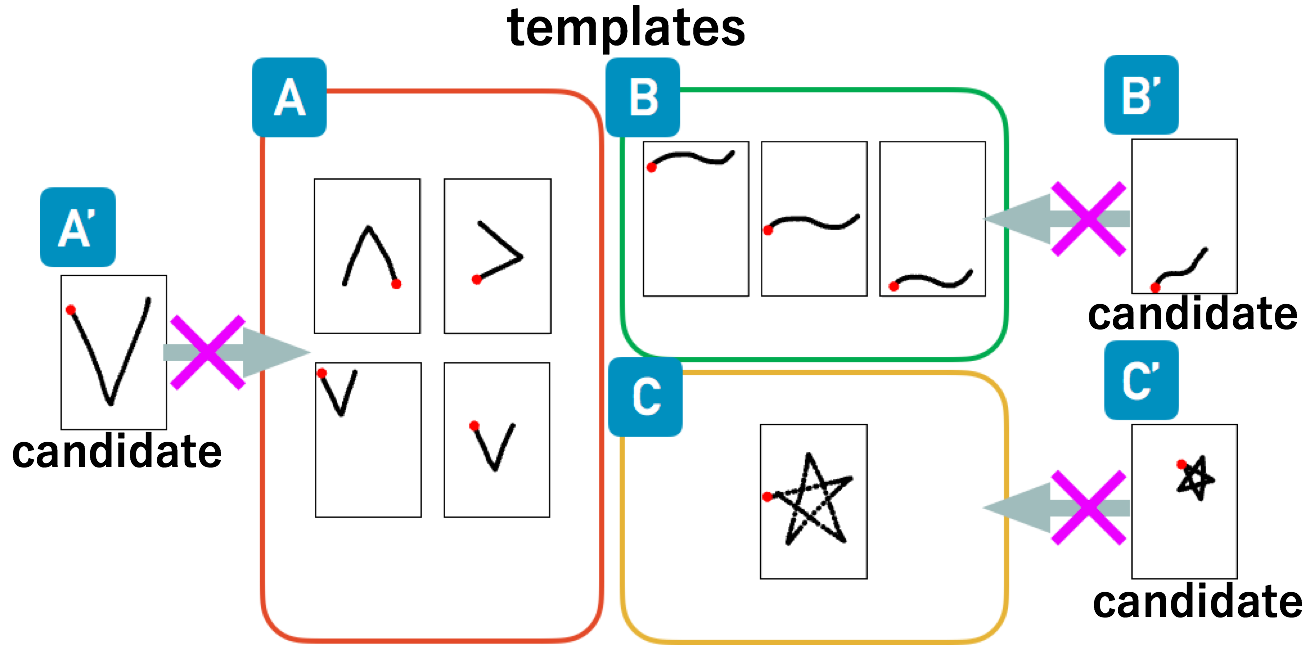
\includegraphics [width=0.9\hsize ]{img/cannot_recognized.eps}
	\end{center}
	\caption{大きさ,向き,位置を特徴量として認識のために用いた場合に,入力データと学習データが一致しない例}
	\label{fig:cannot_recognized}
\end{figure}

そのため,\$Vでは,大きさ,向き,位置を認識のための特徴量として単に用いるのではなく,
ジェスチャグループごとに,大きさ,向き,位置のうちどの特徴量を認識に用いるか選ぶ,つまり,識別するために必要な特徴量を選ぶ
という処理を施すことによって,認識率の低下を防ぐことが可能となると考えた.

\subsubsection{ジェスチャグループごとの特徴量の選定}
ジェスチャグループごとに,大きさ,向き,位置のうちどの特徴量を用いるかを選ぶための方法を述べる.

\$Vの目的は,ジェスチャの形状と書き順が同じであるが,大きさ,向き,位置に関して識別可能にすることである.つまり,同一ジェスチャグループにおいて,大きさ,向き,位置のいずれかあるいはすべてが異なるジェスチャを識別できれば良い.

ここで,図\ref{fig:cannot_recognized}Aの場合について考える.
図\ref{fig:cannot_recognized}Aのジェスチャグループには,ジェスチャの大きさはどの学習データも同じであるが,向きや位置が異なるジェスチャが存在している.つまり,これらを識別するためには,向き,位置を特徴量として認識に用いることが必要となる.反対に,大きさは特徴量として認識に用いる必要がない.

図\ref{fig:cannot_recognized}Bのジェスチャグループには,ジェスチャの大きさや向きはどの学習データも同じであるが,位置が異なるジェスチャが存在している.つまり,これらを識別するためには,位置を特徴量として認識に用いることが必要となる.大きさや向きは特徴量として認識に用いる必要がない.

図\ref{fig:cannot_recognized}Cのジェスチャグループには,1種類のジェスチャしか存在していない.つまり,識別のためにいずれの特徴量も認識に用いる必要がない.

このようにして,ジェスチャグループに存在する学習データの種類によって,認識に用いる特徴量を選ぶ,つまり,ある特徴量については認識のために特徴量として用いないことによって,その特徴量について不変にし,ロバスト性を維持する.これにより認識率の低下を防ぐことが可能となる.

以上を踏まえ我々は,「同一ジェスチャグループ内において,他の学習データと類似している特徴量は,認識のための特徴量として用いなければ,認識率の低下を抑えることができる」という仮説を立てた.

\section{認識に用いる特徴量を選定した時の認識率と認識速度の実験}
前節までにおいて述べてきたように,ジェスチャグループを作成し,ジェスチャグループ内に存在する学習データのみに対し,大きさ,向き,位置の類似度計算をすると認識速度の低下を抑えることができるという仮説と,
同一ジェスチャグループ内において,他の学習データと類似している特徴量は,認識のための特徴量として用いなければ,認識率の低下を抑えることができるという仮説を検証するための実験を行った.
ここではまず,実験を行うにあたって,大きさ,向き,位置,それぞれの特徴量と類似度の定義,ジェスチャグループの作成方法,ジェスチャグループにおける認識に用いる特徴量の選定方法をそれぞれ具体的に述べてから,実験の内容を述べる.

\subsection{ジェスチャの特徴量と類似度の定義}
ジェスチャの大きさ,向き,位置を特徴量として用いた時の,それぞれの特徴量と類似度の定義を示す.

\subsubsection{大きさ}
ジェスチャを構成するストロークの点を内包するように隣接した矩形の面積をジェスチャの大きさとして定義する (図).
学習データと入力データの類似度$S_\textit{s}$を式5.1によって定義する.
\begin{equation}
S_\textit{s} = \left \{
\begin{array}{l}
\frac{S'}{S} (S>S') \\\\
\frac{S}{S'} (S'>S')
\end{array}
\right.
\end{equation}
ここで,Sは入力データの矩形の面積,S'は学習データの矩形の面積である.

\subsubsection{向き}
ジェスチャを構成するストロークの始めの点の座標,全サンプル点の中心座標,その中心座標から右横に延長した線(0度)によって形成させる角度をジェスチャの向きとして定義する(図\ref{fig:angle}).
そして学習データと入力データの類似度$S_\textit{o}$を式5.2によって定義する.
\begin{equation}
S_\textit{o} = 1 - \frac{|\theta - \sigma|}{\pi}
\end{equation}
ここで,$\theta$は入力データの向き,$\sigma$は学習データの向きである.


\subsubsection{位置}
ジェスチャを構成するストロークのすべての点の中心座標をジェスチャの位置として定義する(図\ref{fig:location}).
そして学習データと入力データの類似度$S{\scriptsize p}$を式5.3によって定義する.
\begin{equation}
S_\textit{p} = 1 - \frac{\sqrt{(x - x')^2 + (y - y')^2}}{\sqrt{W\!idt\!h^2 * H\!ei\!ght^2}}
\end{equation}
ここで,(x, y)は入力データの位置,(x', y')は学習データの位置であり,Widthは入力領域全体の横,Heightは縦の長さである.

\subsection{ジェスチャグループの作成方法}
ジェスチャの形状と書き順が同じ学習データが集まったグループである,ジェスチャグループを作成するための手順を以下に示す.
まず,学習データが新たに追加される場面を考える.
\begin{enumerate}
\renewcommand{\labelenumi}{\Alph{enumi}.}
\item 同じ名前の学習データが存在する場合

%同じジェスチャとして管理される.
新たに追加された学習データは同じ名前の学習データと一緒に保管される.この時,その名前を持つ学習データの,大きさ,向き,位置の特徴量は,それぞれの特徴量の算術平均によって表される.\TODO{図を入れる}
 
\item 同じ名前の学習データが存在しない場合\TODO{全体的に図を入れる}

\$1アルゴリズムを用いることによりジェスチャの形状と書き順を判断し,

\begin{enumerate}
\renewcommand{\labelenumi}{\alph{enumi}.}

\item 同じ形状と書き順のジェスチャグループが存在しない場合
 
%別の形状のジェスチャのグループとして管理される
新たに追加された学習データは新しい,ジェスチャグループとして保管される.
   
\item 同じ形状と書き順のジェスチャグループが存在する場合

%次節にて詳細を述べる.
そのジェスチャグループに保管される.

\end{enumerate}
\end{enumerate}

ここで,新たに追加された学習データが,既存のジェスチャグループに対し形状と書き順が同じかどうかを判別する方法は,既存のジェスチャグループ内の学習データ1つ1つと比較することによって行う.今回は\$1による類似度が0.8を超えたときに,形状と書き順が同じであると判断した.これは\$1アルゴリズムにて,類似度のN-best Listの1番目と2番目の差が0.2以上であることを利用している(図\ref{fig:n-bestlist}).ここで,類似度のN-best Listとは,N 個の学習データそれぞれに対するテストデータとの類似度を降順に並べたもの,1番目と2番目の差が大きいほど識別性能が高いことを示す.もし1つでも形状と書き順が同じジェスチャが存在すれば,そのジェスチャが存在するジェスチャグループに保管される.なお,保管候補のジェスチャグループが複数存在する場合は,最も類似度が高かったジェスチャが存在するジェスチャグループに保管される.


\subsection{ジェスチャグループにおける認識に用いる特徴量の選定方法}
我々は,同一ジェスチャグループ内において,他の学習データと類似している特徴量は,認識のための特徴量として用いなければ,認識率の低下を防ぐことができるという仮説を立てた.
ここで,同一ジェスチャグループ内における他の学習データとの類似度を``ジェスチャグループの学習データ間の類似度''とし,その定義を以下のように定める.

まず,同一ジェスチャグループ内において,学習データを2つずつ抽出し,それぞれのペアについて学習データどうしの大きさ,向き,位置の類似度を式5.1〜式5.3を用いて求める.そして,各ペアにおける類似度を比較した時に,それぞれの特徴量について,最小となった類似度を,その形状グループの学習データ間のそれぞれの特徴量についての類似度とする.

例えば,図\ref{fig:group_similarity}左に示すジェスチャグループの場合,同一ジェスチャグループ内に4つの学習データが存在する.そのため,2つずつ抽出した場合の学習データの組み合わせは{\scriptsize 4}C{\scriptsize 2}=6通り存在する~(図\ref{fig:group_similarity}右).それぞれのペアについて,学習データどうしの大きさ,向き,位置の類似度はそれぞれのペアにおいて図\ref{fig:group_similarity}右示されている.この時それぞれの類似度の最小値は,大きさは0.8,向きは0.1,位置は0.4となるため,このジェスチャグループの学習データ間の類似度は~(大きさ,向き,位置) =~(0.8, 0.1, 0.4)となる~(図\ref{fig:group_similarity}左).
ここで,類似度の最小値を用いる理由は,類似度が小さいということは,その特徴量に関して類似していないことを示し,類似していない学習データの組み合わせが1つでも存在すれば,その特徴量について識別するために,認識のための特徴量として用いる必要があると考えたからである.

\begin{figure} [h!]
	\begin{center}
		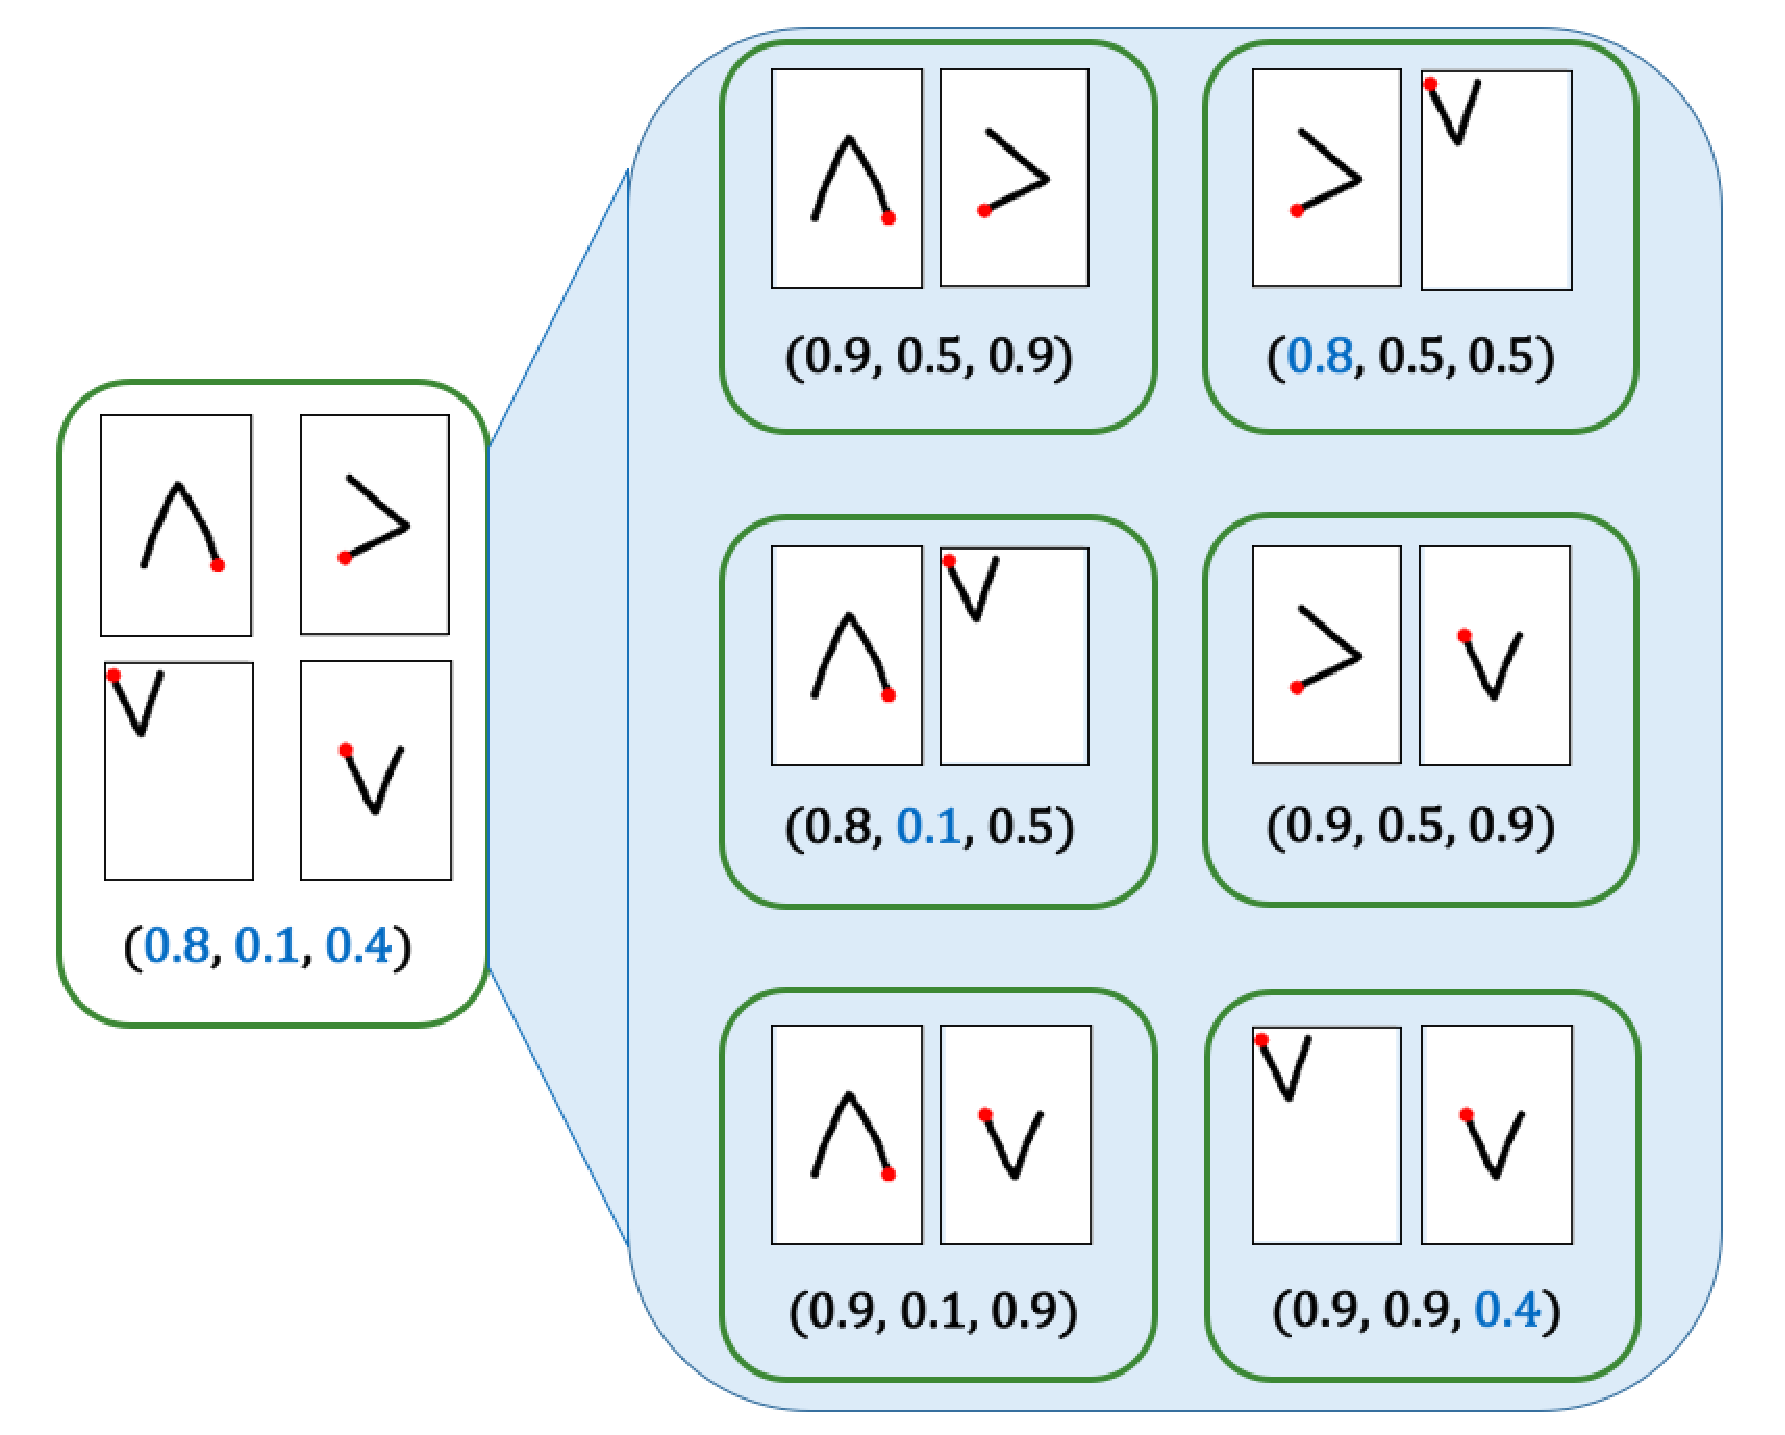
\includegraphics [width=0.8\hsize ]{img/group_similarity.eps}
	\end{center}
	\caption{ジェスチャグループの学習データ間の類似度~($Sts$, $Sto$, $Stp$) を求める方法,この場合,(0.8, 0.1, 0.4)となる.}
	\label{fig:group_similarity}
\end{figure}

以上のようにして得られたジェスチャグループの学習データ間の類似度を用いて,そのジェスチャグループが認識に用いる特徴量を選定する.本実験においては,類似度が0.2を下回った特徴量を,認識に用いる特徴量として選定した.


\subsection{ジェスチャの認識方法}
入力データの認識方法の手順は2つに分かれている.
\begin{enumerate}
\item \$1アルゴリズムを用いることにより,どのジェスチャグループに属するか判別する.この時,学習データを追加する時と同様,ジェスチャグループ内のすべての学習データに対し類似度を求め,0.8を超えた場合あるいは,0.8を超えるジェスチャが複数存在する場合は,最も類似度が高いジェスチャが存在するジェスチャグループに属すると判別する.
\item 1.によって判別されたジェスチャグループ内において,どのジェスチャと最も類似しているかを判別する.
\end{enumerate}
2. において,類似度$S_\textit{final}$は以下の式によって求められる.
\begin{equation}
S_\textit{final} = \frac{S_\textit{cs} \times α_\textit{s} + S_\textit{co} \times α_\textit{o} + S_\textit{cp} \times α_\textit{p}}{n}
\end{equation}

\begin{equation}
α_\textit{s}= \left \{
\begin{array}{l}
1 (S_\textit{ts}<0.2) \\\\
0 (else)
\end{array}
\right.
\end{equation}

\begin{equation}
α_\textit{o}= \left \{
\begin{array}{l}
1 (S_\textit{to}<0.2) \\\\
0 (else)
\end{array}
\right.
\end{equation}

\begin{equation}
α_\textit{p} = \left \{
\begin{array}{l}
1 (S_\textit{tp}<0.2) \\\\
0 (else)
\end{array}
\right.
\end{equation}

ここで,$S_\textit{cs}$は入力データと学習データの大きさの類似度,$S_\textit{co}$は入力データと学習データの向きの類似度,$S_\textit{cp}$は入力データと学習データの位置の類似度を示しており,$S_\textit{ts}$は学習データ間の大きさの類似度,$S_\textit{to}$は学習データ間の向きの類似度,$S_\textit{tp}$は学習データ間の位置の類似度を示している.また,nは1となる$α_\textit{s}$,$α_\textit{o}$,$α_\textit{p}$の数であり,0 $\leq$ n $\leq$ 3を満たす正の整数である.なお,n = 0の時,$S_\textit{final}$は計算せず,手順1.において,最も類似度が高いジェスチャを一致するジェスチャとして判別する.

\subsection{被験者}
被験者は,ユーザ調査において協力してもらった6名である~(男性6名,21〜27歳~(平均23.8歳),全員右利き).

\subsection{実験機器}
実験には,入力端末としてiPhone5を用い,実験における入力領域は1.94'' × 3.18''であり,解像度は640 × 1036である~(図\ref{fig:screenshot}における緑色の部分).

\begin{figure}[!h]
\centering
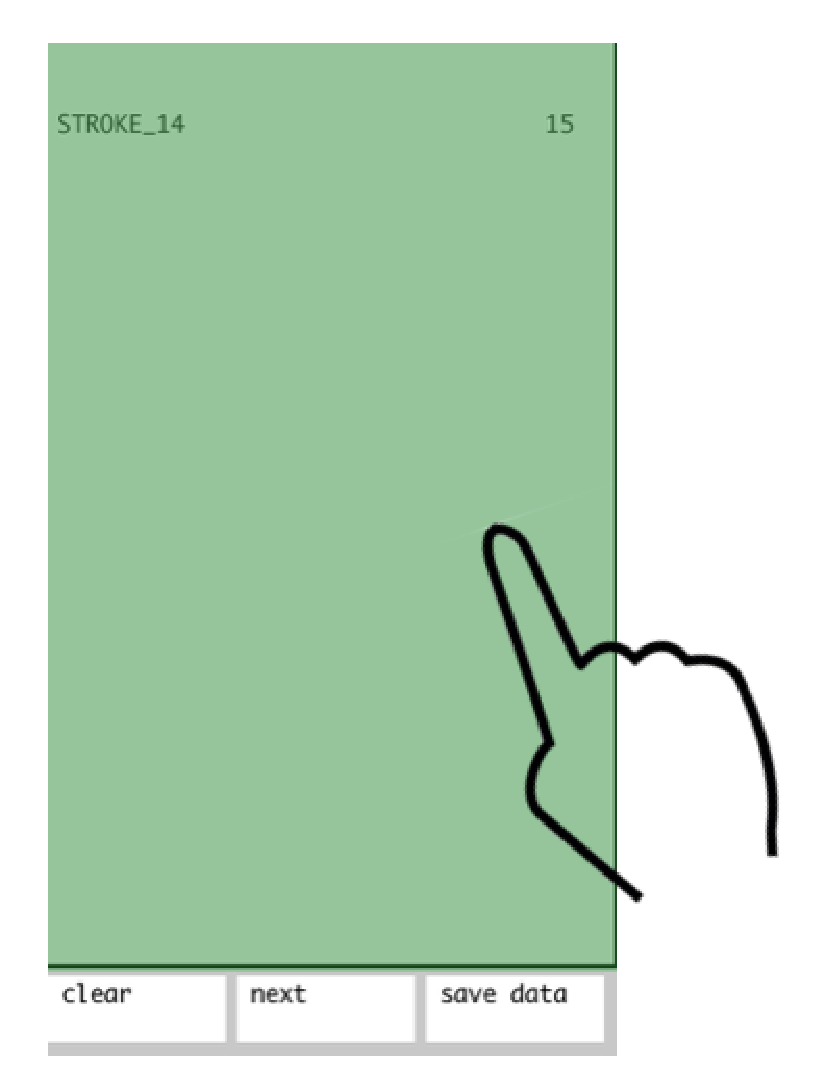
\includegraphics[width=0.4\columnwidth]{img/screenshot.eps}
\caption{実験に用いたスマートフォンのスクリーンショット.緑色のエリアがジェスチャが入力されるエリアである.}
\label{fig:screenshot}
\end{figure}


\subsection{実験手順}
\subsubsection{ジェスチャの取得}
我々はまず,被験者に実験の目的を説明した.
その後,ユーザ調査において記入してもらった紙を見ながら,自身が入力したそれぞれのジェスチャを入力するよう指示した.
この,それぞれの被験者ごとのジェスチャを``ジェスチャセット''とする.
ジェスチャは図\ref{fig:screenshot}における緑色の領域部分にジェスチャを入力するよう指示した.
その際,そのジェスチャを入力するときの姿勢が紙に書かれているため,それに従い入力するよう指示した.
それぞれのジェスチャセットにおいて,ジェスチャには,ジェスチャ番号がSTROKE\_1のようにして割り振られており,図\ref{fig:screenshot}に示すように,画面左上に入力すべきジェスチャが表示される.
タスクの1試行は被験者が1つのジェスチャを入力するまでである.被験者はランダムに選択されたそれぞれのジェスチャを1回ずつ入力し,自身のジェスチャセットに含まれるジェスチャ全てを入力し,これを1セッションとした.これを10セッション行った.被験者によって入力すべきジェスチャの数は異なるが,いずれの被験者においても20以上のジェスチャを入力する(20〜24個のジェスチャ,平均22個).したがって,被験者は平均して計220試行~(22ジェスチャ $\times$ 10セッション)行った.
ジェスチャが思うように入力できなかった場合には,何度でも書き直し可能とした.

\subsubsection{認識率と認識速度の測定}
本実験において被験者は6人であるため,ジェスチャセットは6つ存在する.実験は各被験者が自身のジェスチャセットについてのみ行うためユーザ依存となる.それぞれのジェスチャは10個ずつあり,学習データをランダムにE個選ぶ.その際のジェスチャグループの決め方と,ジェスチャグループの学習データ間の類似度の計算方法は,5.3.2節及び5.3.3節に示したとおりである.学習データを追加し終わった後,入力データを残りの10 - E個のジェスチャからランダムに1個選び,認識率と認識速度を測定した~(10分割交差検定).これをそれぞれのジェスチャにつき100回行った.本実験はE = 1〜5とした.また,認識率はジェスチャセットにおける認識率の100回平均を学習データごとに測定し,認識速度は,ジェスチャ1つを認識し終わるまでに要した時間のジェスチャセットに含まれる全ジェスチャの平均値の100回平均であり,テストに用いるジェスチャをランダムに選ぶ過程は含まれていない.

\subsubsection{N-best Listの1番目と2番目の差と類似度の測定}
認識率と認識速度に加え,類似度のN-best Listの1番目と2番目の差及び類似度の測定も行う.ここで,類似度のN-best Listとは,ある入力データが,全ての種類の学習データに対してどれくらい類似しているかを示すものであり,1番目と2番目の差が大きいほど識別性能が高いことを示す.また,本実験においては,正しく認識されたジェスチャの類似度の平均値の100回平均,正しく認識されたジェスチャのうち,類似度が最も低かったものの100回平均も測定した.


\subsection{実験結果と考察}
それぞれの被験者ごとの認識率,認識速度,N-best Listsの1番目と2番目の差,ジェスチャが正しく認識された時の類似度,ジェスチャが正しく認識された時の類似度の最小値を示す.

上記の結果について,正規化せずにリサンプリングした点のみによってジェスチャを比較する場合及び,ジェスチャグループごとに特徴量を認識に用いるが選定しない手法,つまり,どのジェスチャグループに対しても大きさ,向き,位置の特徴量を類似度に用いる手法についても併せて示す.

\subsubsection{認識率}
\begin{figure}[!h]
\centering
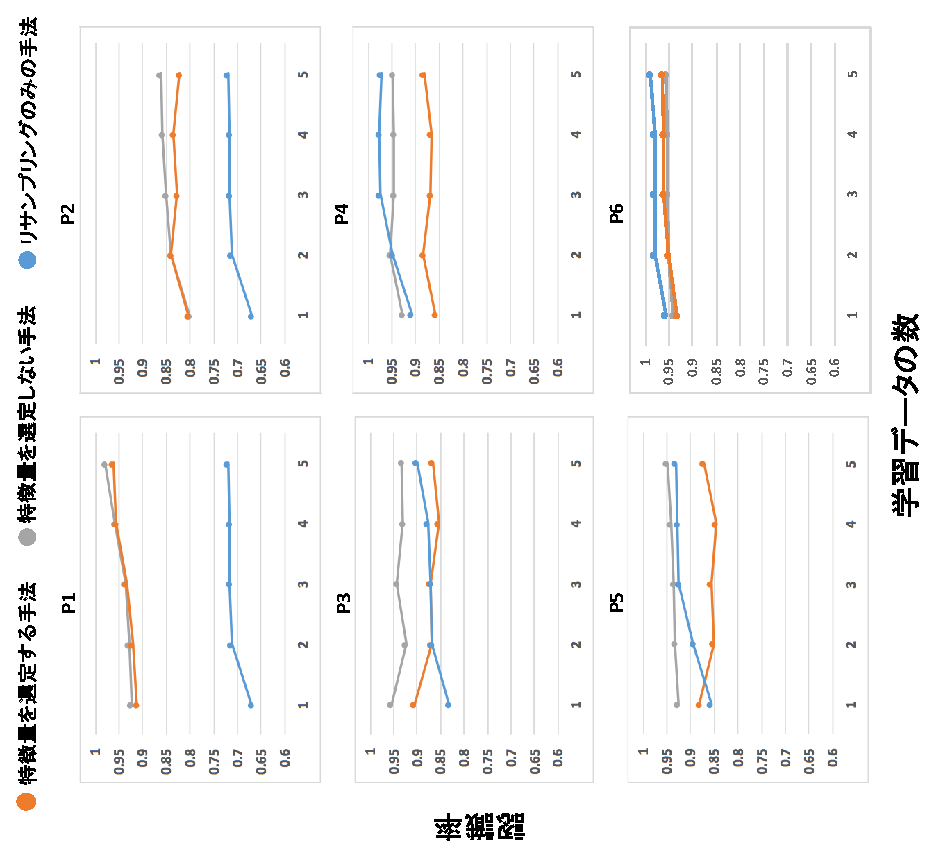
\includegraphics[width=1.0\columnwidth]{img/pre_rec.eps}
\caption{各手法における,被験者ごとの認識率}
\label{fig:rare_rec}
\end{figure}

特徴量を選定する手法及び特徴量を選定しない手法は,どの被験者のジェスチャセットにおいても認識率は高かった.
リサンプリングのみの場合は,ジェスチャセットによっては認識率は低かった.
また,リサンプリングのみの手法は,学習データの数に比例して認識率が高くなったが,特徴量を選定する手法及び特徴量を選定しない手法において,認識率は必ずしも学習データの数と認識率は比例しなかった.

これは,リサンプリングのみの手法は,学習データが増えるほど,入力データに類似する学習データが存在する可能性が高くなるが,特徴量を選定する手法及び特徴量を選定しない手法は,同じジェスチャの学習データを追加するたびに,大きさ,向き,位置それぞれの特徴量を算術平均するため,必ずしも入力データに類似する学習データが存在する可能性が高くなるとは言えないからである.

\subsubsection{認識速度}
\begin{figure}[!h]
\centering
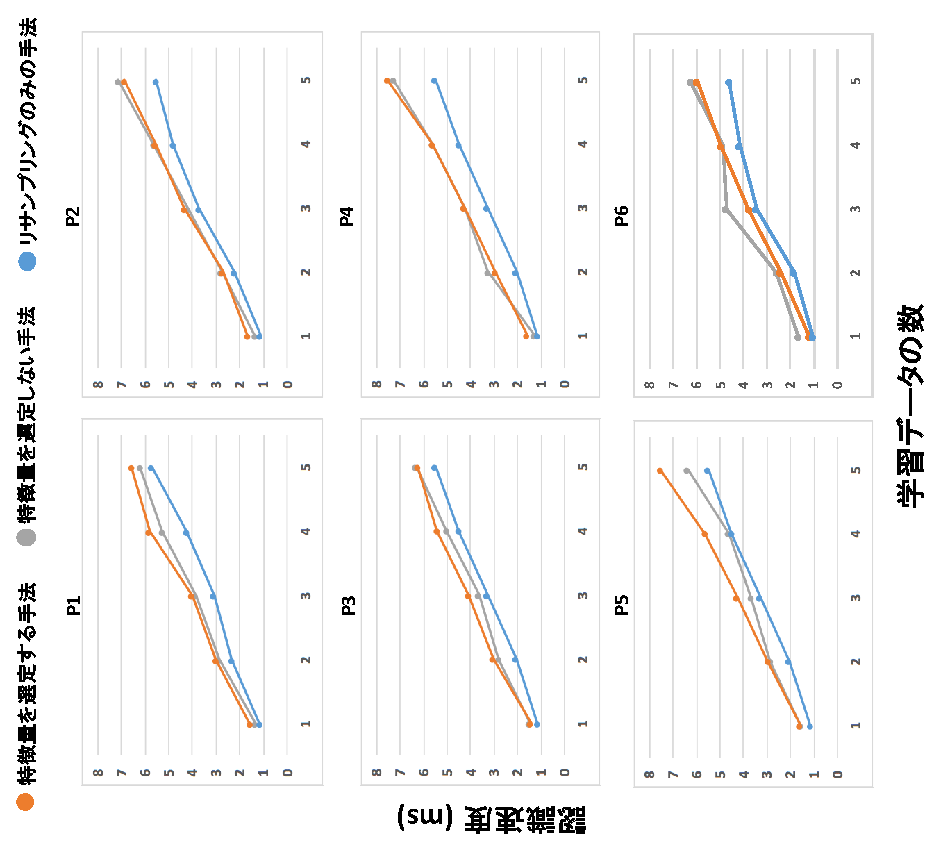
\includegraphics[width=1.0\columnwidth]{img/pre_speed.eps}
\caption{各手法における,被験者ごとの認識速度}
\label{fig:rare_rec}
\end{figure}

いずれの手法においても,認識速度はほとんど変わらなかった.リサンプリングのみの手法は,正規化処理を行わないため,最も認識速度は速くなった.特徴量を選定しない手法は,正規化したのち,特徴量を選定するための処理を行わないため次に認識速度が速くなった.特徴量を選定する手法は正規化に加え,特徴量を選定する処理を行う必要があるため最も認識速度が遅くなった.また,どの場合においても認識速度は学習データの数に比例して遅くなった.

\subsubsection{N-best Listsの1番目と2番目の差}
\begin{figure}[!h]
\centering
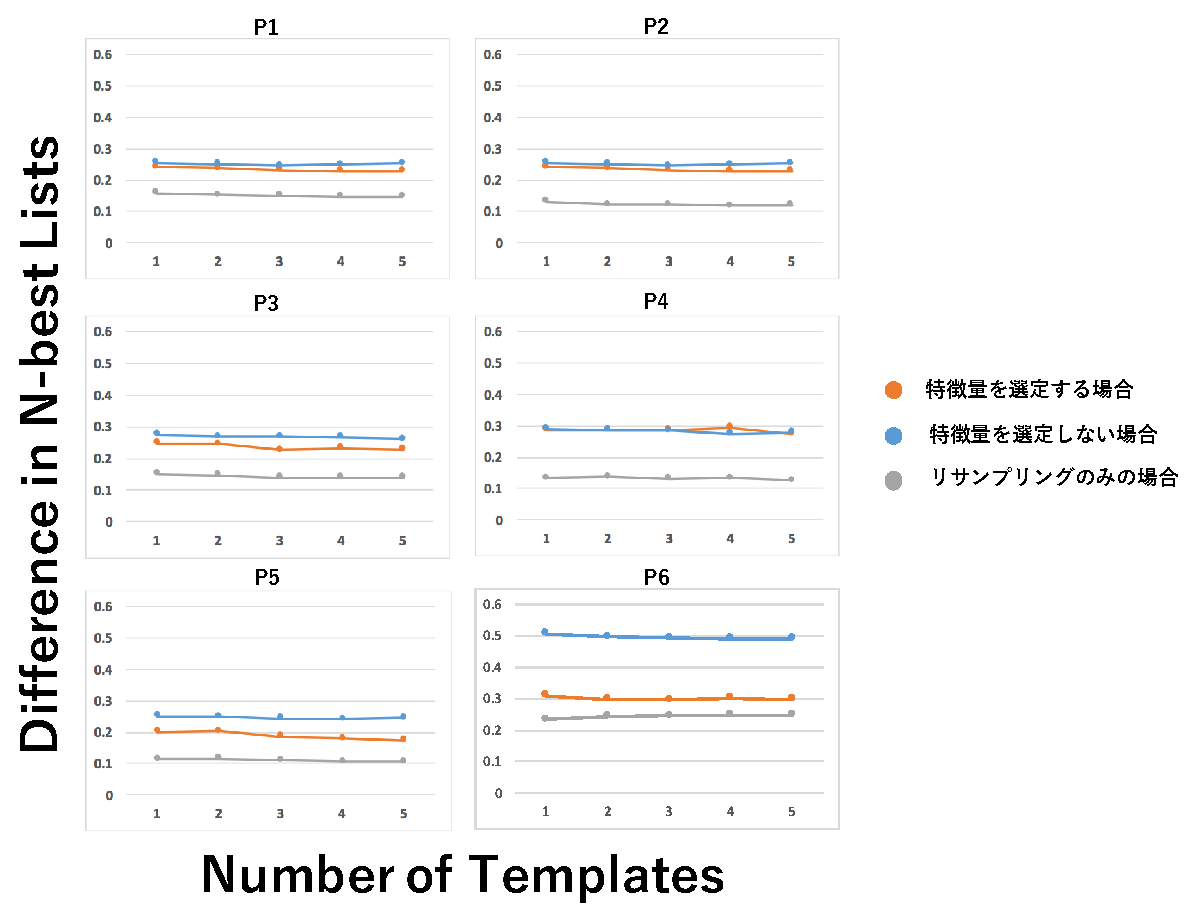
\includegraphics[width=1.0\columnwidth]{img/pre_diff.eps}
\caption{各手法における,被験者ごとのN-best Listsの1番目と2番目の差}
\label{fig:rare_rec}
\end{figure}

N-best Listsの1番目と2番目の差は,リサンプリングのみの手法,特徴量を選定する手法,特徴量を選定しない手法の順に大きくなった.
リサンプリングのみの場合においては,正規化しないため,類似するジェスチャとそれ以外のジェスチャにおいて,類似度の差が大きくなりやすくなったと言える.特徴量を選定する手法及び特徴量を選定しない手法は,正規化するため,類似度の差が大きくなりづらいが,特徴量を選定する手法は,ジェスチャグループの学習データ間の類似度が小さい特徴量のみ認識に用いているため,類似度の差が比較的大きくなったと言える.それに対し,特徴量を選定しない手法は識別に必要のない特徴量も認識に用いるため,例えば,向きが異なるが位置がほぼ同じであるジェスチャを識別しようとする場合に,位置の類似度を加味してしまうため,類似度の差が小さくなったと言える.

\subsubsection{ジェスチャが正しく認識された時の類似度}
\begin{figure}[!h]
\centering
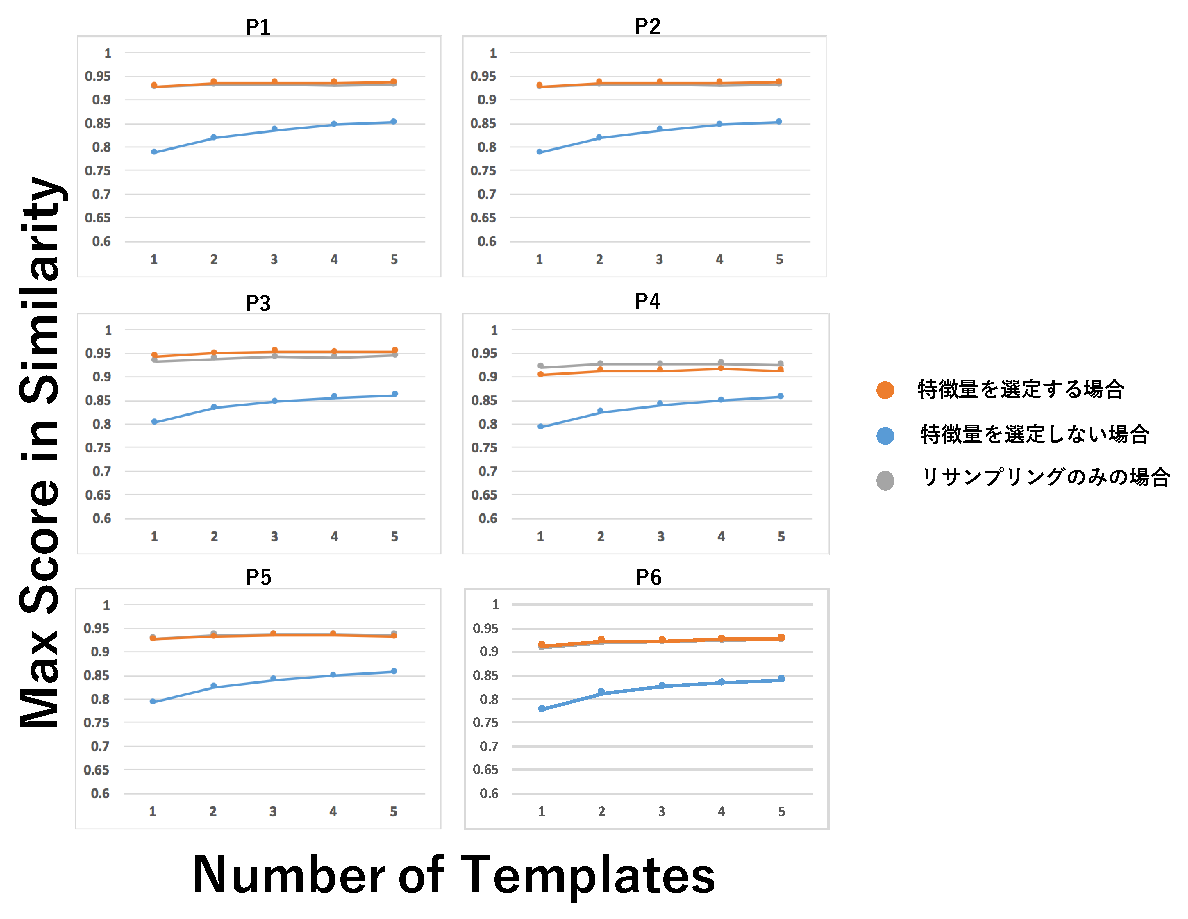
\includegraphics[width=1.0\columnwidth]{img/pre_sim.eps}
\caption{各手法における,被験者ごとのジェスチャが正しく認識された時の類似度}
\label{fig:rare_rec}
\end{figure}

特徴量を選定する手法及び特徴量を選定しない手法は,ジェスチャが一致した時の類似度の平均値は高くなり,ほぼ同じような結果となった.特徴量を選定しない手法は,特徴量を選定する場合と比べて類似度が小さくなると予想されたが,このような結果となった.これは,本実験がユーザ依存であったため,被験者の書くジェスチャの再現率が高かったことが原因であると言える.リサンプリングのみの手法は被験者の書くジェスチャの再現率が高くとも,正規化しないため類似度が低くなったと言える.

\subsubsection{ジェスチャが正しく認識された時の類似度の最小値}
\begin{figure}[!h]
\centering
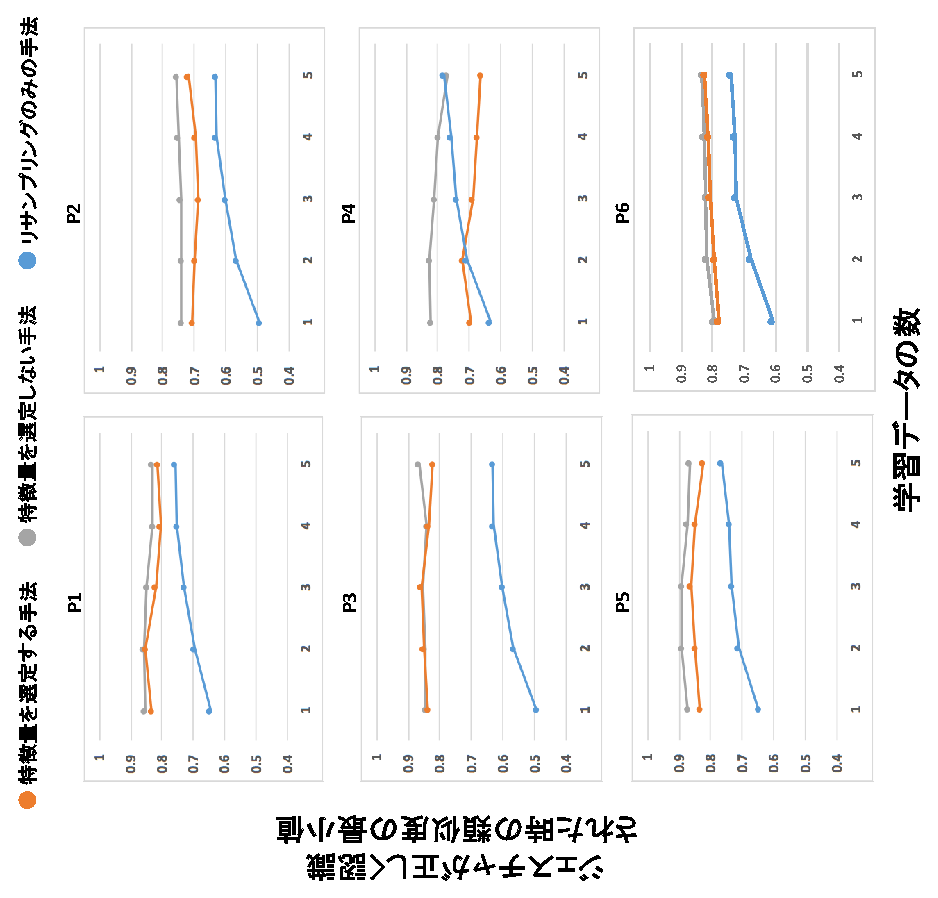
\includegraphics[width=1.0\columnwidth]{img/pre_min.eps}
\caption{各手法における,被験者ごとのジェスチャが正しく認識された時の類似度の最小値}
\label{fig:rare_rec}
\end{figure}

特徴量を選定する手法及び特徴量を選定しない手法は,ジェスチャが一致した時の類似度の最小値は高くなった.また,リサンプリングのみの手法は低くなった.これらの要因は,ジェスチャが一致した時の類似度と同様であると考えられる.

\subsection{議論}

特徴量を選定する手法及び特徴量を選定しない手法はいずれも,認識率,認識速度のスコアは高く,特徴量を選定する手法はN-best Listsの1番目と2番目の差も大きくなった.以上を踏まえ,
ジェスチャグループを作成し,ジェスチャグループ内に存在する学習データのみに対し,大きさ,向き,位置の類似度計算をすると認識速度の低下を抑えることができるという仮説及び,
同一ジェスチャグループ内において,他の学習データと類似している特徴量は,認識のための特徴量として用いなければ,認識率の低下を抑えることができるという仮説はある程度正しいと言える.それらに加え,特徴量を選定することによって,識別性能が向上するということも言える.

しかしながら被験者によっては,認識率及びN-best Listsの1番目と2番目の差のスコアは低くなった.この原因について考察する.

特徴量を選定する手法において,それぞれの特徴量は,認識に用いられるか用いられないかの二通りに分類され,閾値を設けることにより判別してきたが,ランダムに選ばれる学習データによっては,同じジェスチャグループであったとしても,認識に用いられる特徴量が異なる場合があった (閾値によって二通りのいずれかに分類されてしまうため,閾値の設定も難しいといった問題もある).

また,例えば図\ref{fig:group_similarity}において,向き,位置が認識に用いる特徴量として選ばる可能性が高いが,向きは位置に比べ,類似度が小さい組み合わせが存在するため,向きの方が位置よりも識別するための特徴量としてより考慮されるべきではないのかという疑問や,それぞれの特徴量による類似度を,同じ尺度において扱うことができるのかという疑問があった (例えば,大きさの類似度 0.9 と向きの類似度 0.9 は,同じくらい類似していると言えるのかなど).

そこで,これらの問題点に対し,それぞれの特徴量を,認識に用いられるか用いられないかの二通りに分類するのではなく,特徴量に重み付けをすることによって解決しようと試みた.例えば,図\ref{fig:group_similarity}の場合,それぞれの特徴量に対する重みの和が1となる場合,これまでは特徴量を用いるか用いないかであったため,~(大きさ,向き,位置)の重みが~(0,0.5,0.5)であったところを,~(0.1,0.6,0.3)といった具合にする.
このように重みを導入することによって,認識に用いる特徴量をより高い尤度によって決定することを試みた.

そこで,我々は,認識率及びN-best Listsの1番目と2番目の差のスコアを向上させる「最適な重み」を求めることとした.

%\begin{figure} [h!]
%	\begin{center}
%		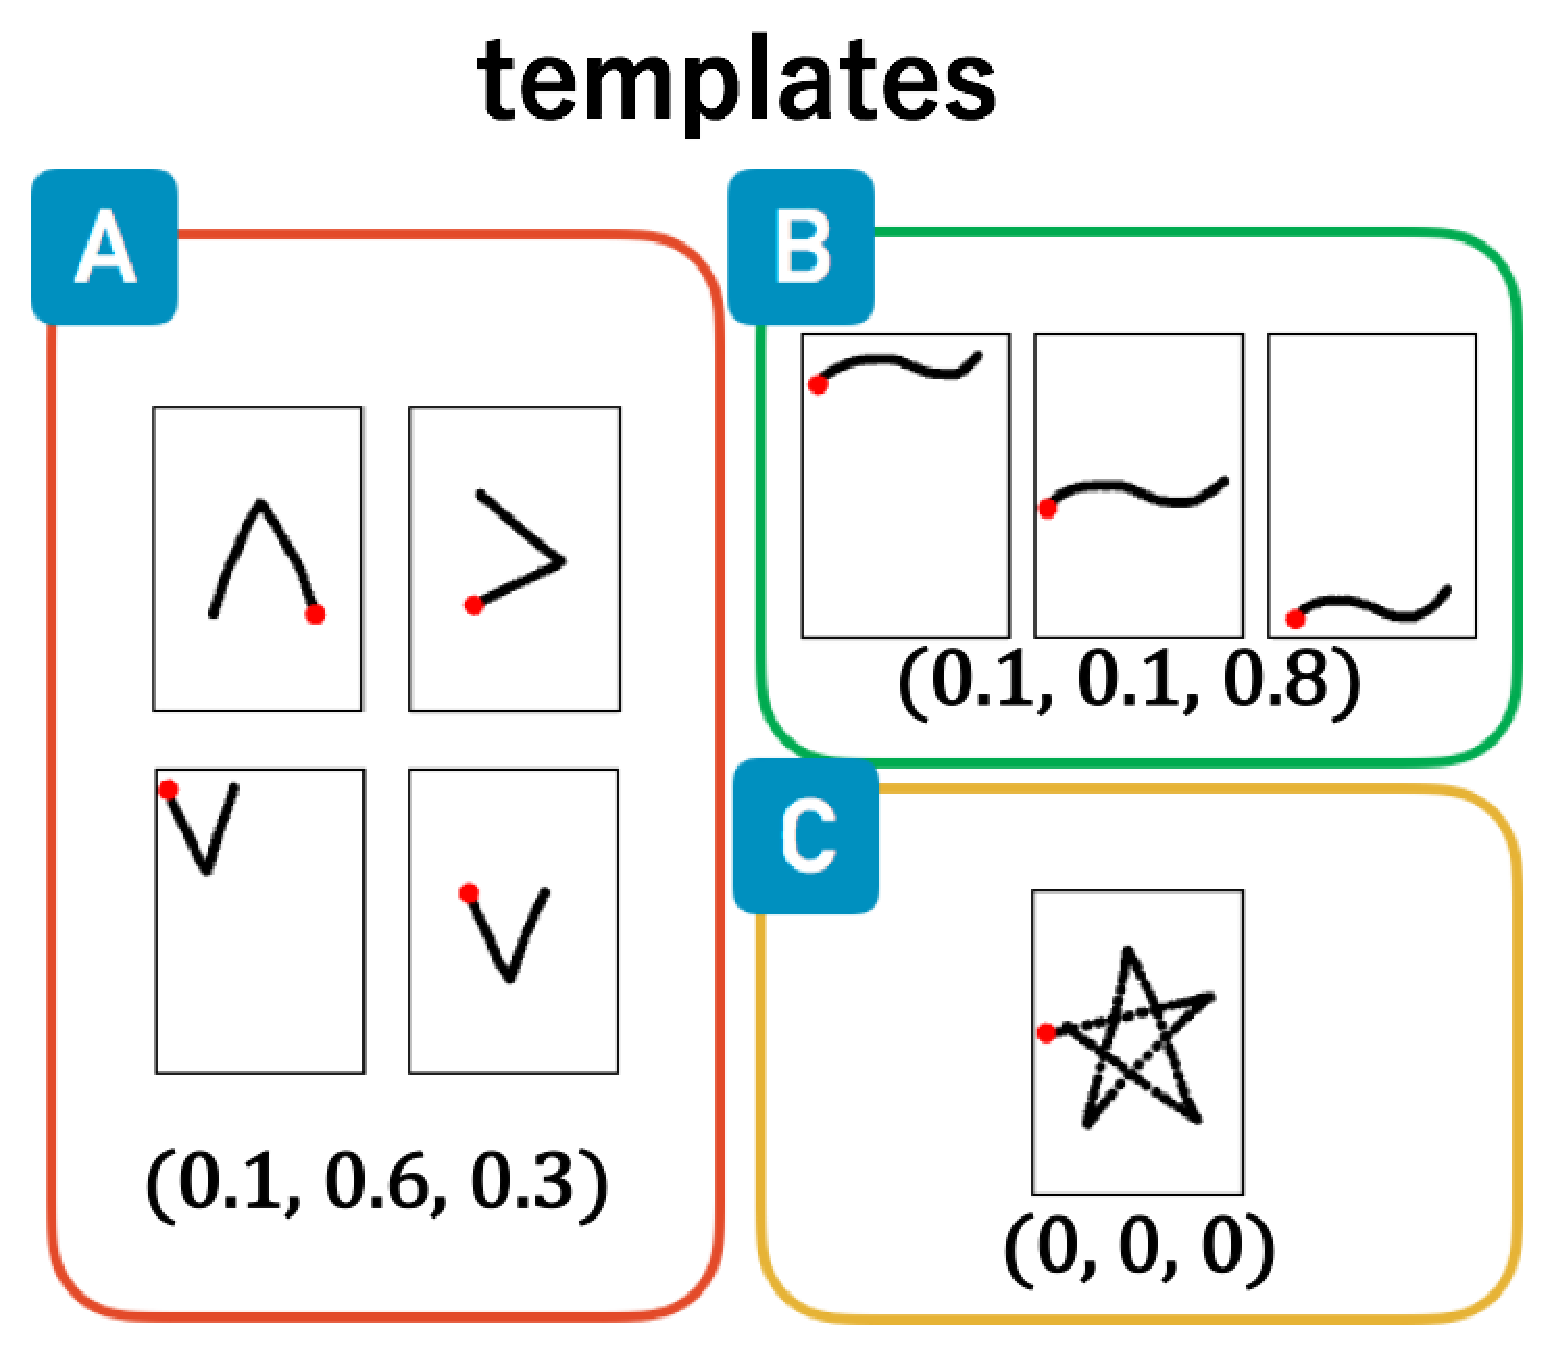
\includegraphics [width=0.7\hsize ]{img/group_weight.eps}
%	\end{center}
%	\caption{Examples of gesture groups and optimal weight values ($Ws$, $Wo$, $Wp$) for each group.}
%	\label{fig:group_weight}
%\end{figure}

\section{最適な重み付けのための実験}
%「同一ジェスチャグループ内において,他の学習データと類似している特徴量は,認識のための特徴量として用いなければ,認識率の低下を防ぐことができる」という仮説
あるジェスチャグループが認識に用いるべき特徴量が,ジェスチャグループの学習データ間の類似度と関係していることは,これまで述べてきた通りである.
そこで我々は,ジェスチャグループの学習データ間の類似度をもとに,認識率及びN-best Listsの1番目と2番目の差のスコアを向上させるためのそれぞれの特徴量に対する最適な重み付けの方法を実験的に求めることとした.

\subsection{重み付けの手順}
重み付けの手順を述べる.

学習データは,追加されるたびに,\$1アルゴリズムを用いてジェスチャグループとして保管される.その際のジェスチャグループの決め方と,ジェスチャグループの学習データ間の類似度の計算方法は,5.3.2節及び5.3.3節に示したとおりである.

全ての学習データを追加し終わった後,入力データを入れていく.
まず\$1アルゴリズムによりどの形状のジェスチャであるかを判定する.
その後,ジェスチャグループにおける大きさ,向き,位置のそれぞれの特徴量に対し,最適な重みを求める方法を図\ref{fig:weight_method1},図\ref{fig:weight_method2}に図示する.
まず,テストデータと学習データの類似度を求める.その後大きさ,向き,位置のそれぞれの特徴量に対する重みを,それぞれの和が1となるようにそれぞれ0.1ずつ変化させていく.そして,重みを先ほど求めた類似度に式〜に則って乗算することによって,最終的な類似度を求める.ここで,式〜において, $S_\textit{cs}$はテストデータと学習データの大きさの類似度,$S_\textit{co}$,はテストデータと学習データの向きの類似度$S_\textit{cp}$はテストデータと学習データの位置の類似度を示しており,$W_\textit{s}$は大きさの重み,$W_\textit{o}$は向きの重み,$W_\textit{p}$は位置の重みを示している.これを各被験者から得られた各ジェスチャセットごとに行う.
この時,ジェスチャが一致した時の類似度の平均値が0.9以上,N-best Listの1番目と2番目の差が0.2以上の時のそれぞれの特徴量に対する重みを最適な重みとして記録する.

そして,それぞれのジェスチャグループ内の学習データ間の類似度と,先ほど記録した重みをセットにして記録することによって,どのような特徴を持つジェスチャグループの場合に,どのような重み付けをすることが望ましいかを考察する.

\begin{equation}
S_\textit{final} = S_\textit{cs} \times W_\textit{s} + S_\textit{co} \times W_\textit{o} + S_\textit{cp} \times W_\textit{p}
\end{equation}

\begin{figure} [h!]
	\begin{center}
		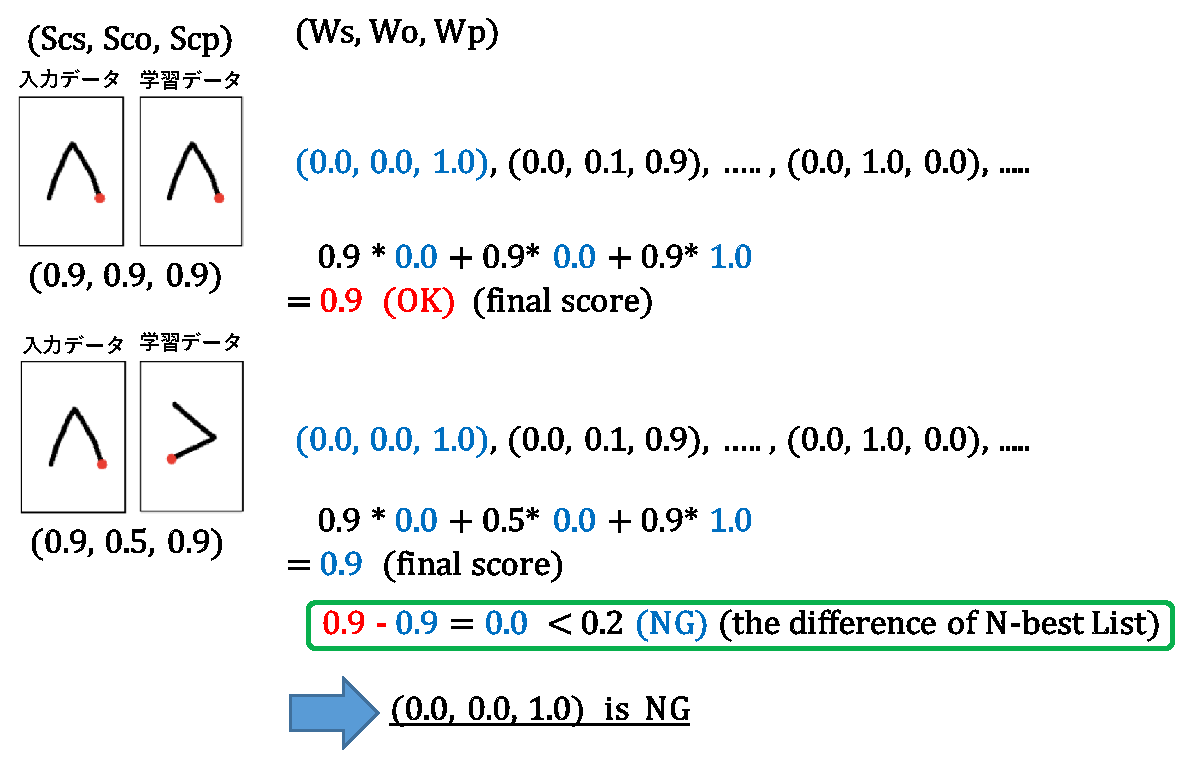
\includegraphics [width=0.8\hsize ]{img/weight_method1.eps}
	\end{center}
	\caption{The procedure to decide the optimal weight values }
	\label{fig:weight_method1}
\end{figure}

\begin{figure} [h!]
	\begin{center}
		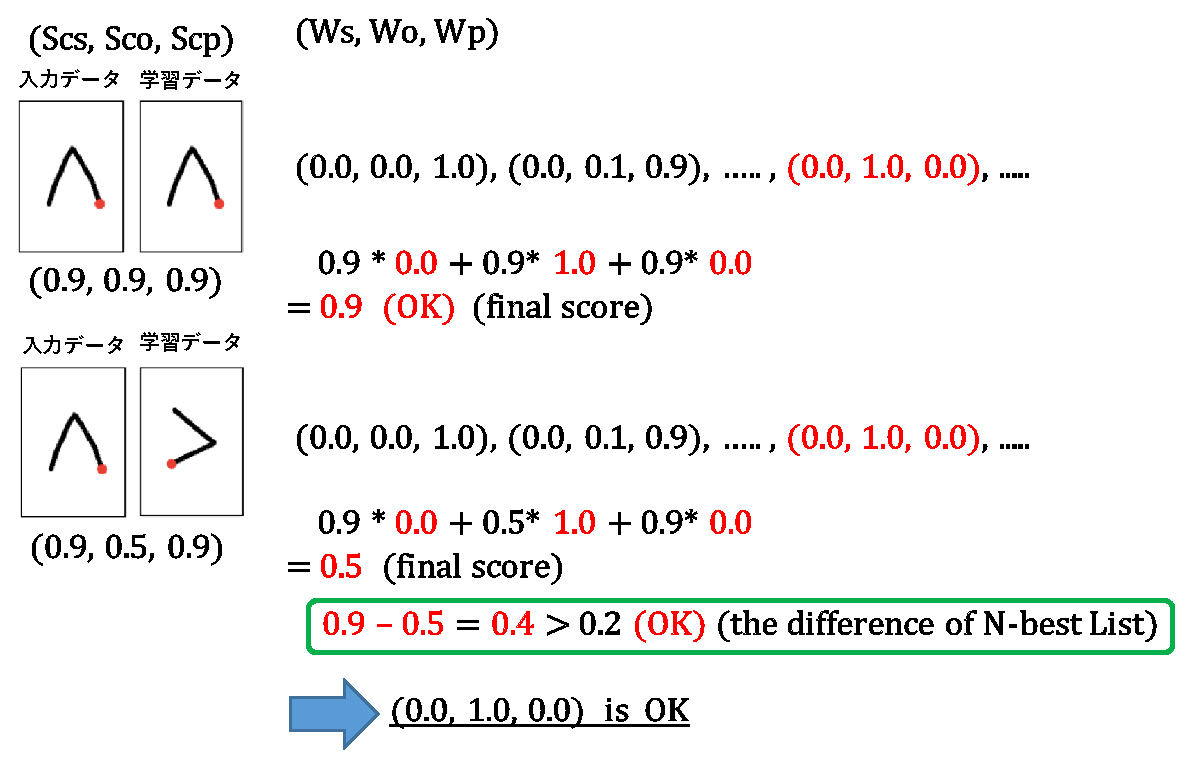
\includegraphics [width=0.8\hsize ]{img/weight_method2.eps}
	\end{center}
	\caption{The procedure to decide non optimal weight values}
	\label{fig:weight_method2}
\end{figure}

\subsection{実験結果}
最適な重み付けのための実験結果を示す.

図\ref{fig:weight_size}は,ジェスチャグループ内の学習データ間の類似度と大きさの最適な重みの関係,
図\ref{fig:weight_orientation},ジェスチャグループ内の学習データ間の類似度と向きの最適な重みの関係,
図\ref{fig:weight_position}は,ジェスチャグループ内の学習データ間の類似度と位置の最適な重みの関係を被験者ごとの結果示している.
ここで,$S_\textit{ts}$は学習データ間の大きさの類似度,$S_\textit{to}$は学習データ間の向きの類似度,$S_\textit{tp}$は学習データ間の位置の類似度を示している.

ある類似度の時の最適な重みは複数存在するため,プロットされているデータは,その平均値と標準偏差である.

\begin{figure}[!h]
\centering
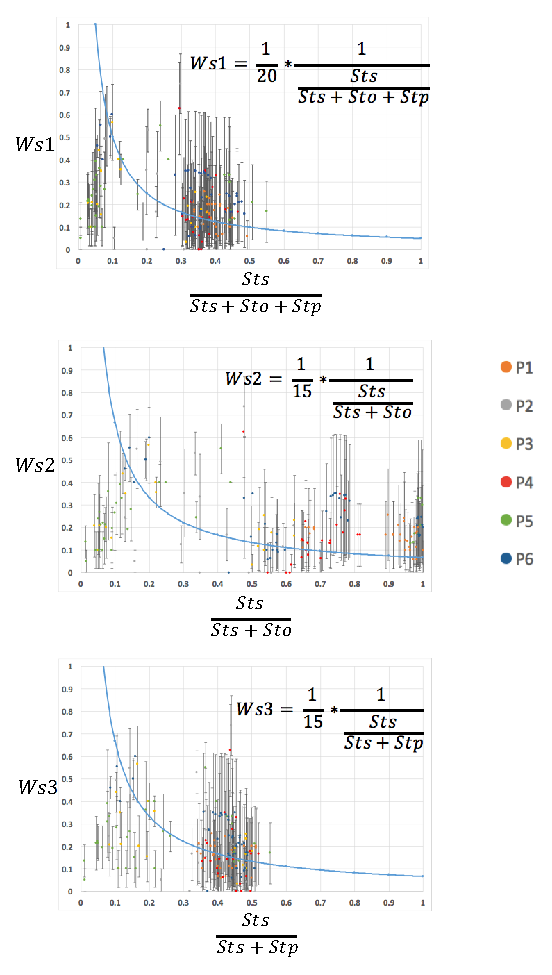
\includegraphics[width=0.7\columnwidth]{img/weight_size.eps}
\caption{The screen shot on the smartphone. The green area is the input area}
\label{fig:weight_size}
\end{figure}

\begin{figure}[!h]
\centering
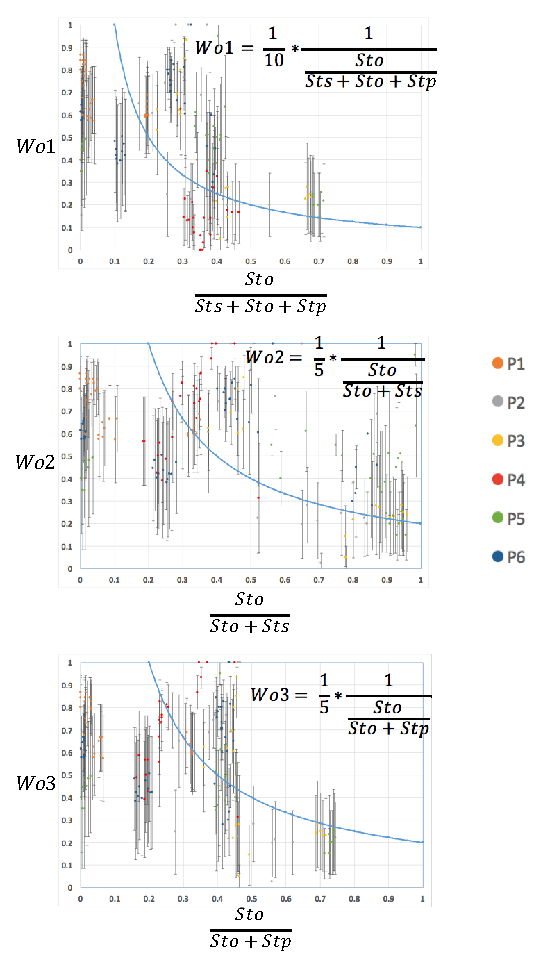
\includegraphics[width=0.7\columnwidth]{img/weight_orientation.eps}
\caption{The screen shot on the smartphone. The green area is the input area}
\label{fig:weight_orientation}
\end{figure}

\begin{figure}[!h]
\centering
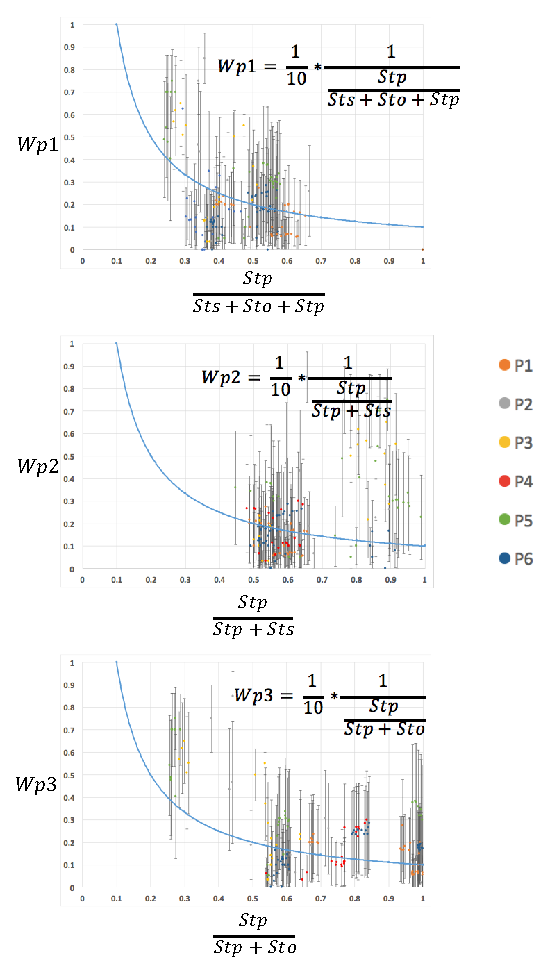
\includegraphics[width=0.7\columnwidth]{img/weight_position.eps}
\caption{The screen shot on the smartphone. The green area is the input area}
\label{fig:weight_position}
\end{figure}

それぞれについて,我々はジェスチャグループ内の学習データ間の類似度と最適な重みを関係式によって表すこととした.
関係式は,それぞれのグラフにおいて青色の線によって示されており,グラフの右上に式が示されている.

この関係式の求め方について述べる.

まず,実験から得られたジェスチャグループ内の学習データ間の類似度と最適な重みの関係の近似式を求める.
この時,両対数グラフにおいて,およそ直線で表せられることがわかった.つまり,これらの関係は累乗近似曲線に近似できることがわかった.
しかしながら,近似曲線に対し離れているデータが多く存在するため,近似式がどれほど元データを表すものになっているかを示す決定係数$R^2$は,どのグラフにおいてもあまり高いとはいえない.

そこで我々は,累乗近似曲線に近似できることを手掛かりに,近似式を以下のように定めた.\begin{equation}
W = \frac{1}{α} \times \frac{1}{S} 
\end{equation}
ここで,Wは重み,Sは類似度を示す.

そして,αを5〜30まで5ずつ増やし,その時に求められる重みを元に認識率を測定したところ,図\ref{fig:weight_size}〜図\ref{fig:weight_position}において示されるような近似式において,認識率が高くなることがわかった.


\section{ジェスチャの認識}
以上を踏まえ,ジェスチャグループ内の学習データ間の類似度を元に,認識率を高くする最適な重みを求めることが可能となる.

まず,学習データを追加する際に,ジェスチャグループ内の学習データ間の類似度を元に最適な重みを求める.
この際,図\ref{fig:weight_size}〜図\ref{fig:weight_position}において示される近似式を元に重みを求める.これは,以下の式に統合される.
\begin{equation}
W_\textit{s} = \frac{1}{90}(5.5 + 3.5\frac{S_\textit{to} + S_\textit{tp}}{S_\textit{ts}})
\end{equation}
\begin{equation}
W_\textit{o} = \frac{1}{30}(5.0 + 3.0\frac{S_\textit{ts} + S_\textit{tp}}{S_\textit{to}})
\end{equation}
\begin{equation}
W_\textit{p} = \frac{1}{30}(5.0 + 3.0\frac{S_\textit{ts} + S_\textit{to}}{S_\textit{tp}})
\end{equation}


次に,実際に入力データを認識させる手順を述べる.
\begin{enumerate}
\item \$1アルゴリズムを用いることにより,どのジェスチャグループに属するか判別する.この時,学習データを追加する時と同様,ジェスチャグループ内のすべての学習データに対し類似度を求め,0.8を超えた場合あるいは,0.8を超えるジェスチャが複数存在する場合は,最も類似度が高いジェスチャが存在するジェスチャグループに属すると判別する.
\item 1.によって判別されたジェスチャグループ内において,どのジェスチャと最も類似しているかを判別する.

この際,ジェスチャグループ内において,入力データと学習データの類似度を求め,学習データを追加した際に求めた最適な重みを用いて式〜によって最終的な類似度を求める.この類似度が最も高かった時のジェスチャが判別されるジェスチャとなる.

\end{enumerate}






